\chapter{Effetto tunnel e decadimento $\alpha$}

Fino a questo punto la costante di decadimento $\lambda$ è stata trattata in due modi diversi. Nel primo capitolo l'abbiamo \emph{postulata}: ogni nucleo ha una probabilità di decadere per unità di tempo costante, e da quell'ipotesi segue l'intera legge esponenziale. Nella sezione sull'interpretazione quantistica l'abbiamo \emph{espressa} attraverso la regola d'oro di Fermi, $\lambda = \frac{2\pi}{\hbar}|V'_{fi}|^2\rho(E_f)$.\\
Quest'ultima espressione, tuttavia, è valida solo quando trattiamo processi perturbativi, cioè processi in cui $V'$ è piccolo rispetto alle altre grandezze in gioco. Nel decadimento $\beta$ la separazione è naturale: l’interazione forte costruisce i livelli, quella debole li fa decadere, e fra le due ci sono venti ordini di grandezza.\\
Nel decadimento $\alpha$ questa separazione non esiste. La stessa forza che tiene la particella dentro la buca, cioè la combinazione di forte e coulombiana, è anche quella che la spinge fuori: non c’è nessun termine aggiuntivo da isolare. Volendo forzare la scrittura, il $V'$ che accoppia lo stato legato a quello libero sarebbe dell’ordine del potenziale nucleare stesso, decine di $MeV$: non una perturbazione. \\
La particella è già presente nel nucleo e deve attraversare una barriera coulombiana che classicamente glielo proibisce. Il problema non è perturbativo ed è governato dall'effetto tunnel.\\

Vedremo anzitutto il dato sperimentale, la legge di Geiger-Nuttall, in cui un intervallo di energie che copre meno di un fattore due corrisponde a tempi di dimezzamento distribuiti su ventiquattro ordini di grandezza. Una dipendenza così violenta non può che essere esponenziale, e lo scopo finale del capitolo è mostrare che quell'esponenziale è la probabilità di attraversare per effetto tunnel la barriera coulombiana.


\section{La legge di Geiger-Nuttall}

Osservando sistematicamente gli emettitori $\alpha$ naturali si trova una regolarità sorprendente, riassunta nella tabella seguente.

\begin{table}[htbp]
\centering
\begin{tabular}{cclccc}
\hline
$Z$ & $A$ & Nuclide & $Q$ [MeV] & $1/\sqrt{Q}$ & $T_{1/2}$ \\
\hline
92 & 238 & U  & $4,27$ & $0,484$ & $4,47 \cdot 10^9$ y \\
92 & 234 & U  & $4,86$ & $0,454$ & $2,46 \cdot 10^5$ y \\
90 & 230 & Th & $4,77$ & $0,458$ & $7,54 \cdot 10^4$ y \\
88 & 226 & Ra & $4,87$ & $0,453$ & $1,6 \cdot 10^3$ y \\
86 & 222 & Rn & $5,59$ & $0,423$ & $3,8$ d \\
84 & 218 & Po & $6,11$ & $0,405$ & $3,10$ min \\
\hline
\end{tabular}
\caption{Energia liberata e tempo di dimezzamento per alcuni emettitori $\alpha$.}
\label{tab:geiger_nuttall}
\end{table}

\newpage

Diagrammando $\log_{10}(T_{1/2}/\mathrm{s})$ in funzione di $1/\sqrt{Q}$ i punti si dispongono su una retta, cioè vale la legge di Geiger-Nuttall\mkeyword{legge di Geiger-Nuttall}

\begin{tcolorbox}[colback=black!5!white, colframe=black!45!white, boxrule=0.8pt]
\begin{equation}
    \ln T_{1/2} = \frac{a}{\sqrt{Q}} + b
    \label{eq:geiger_nuttall}
\end{equation}
\end{tcolorbox}

\begin{figure}[htbp]
\centering
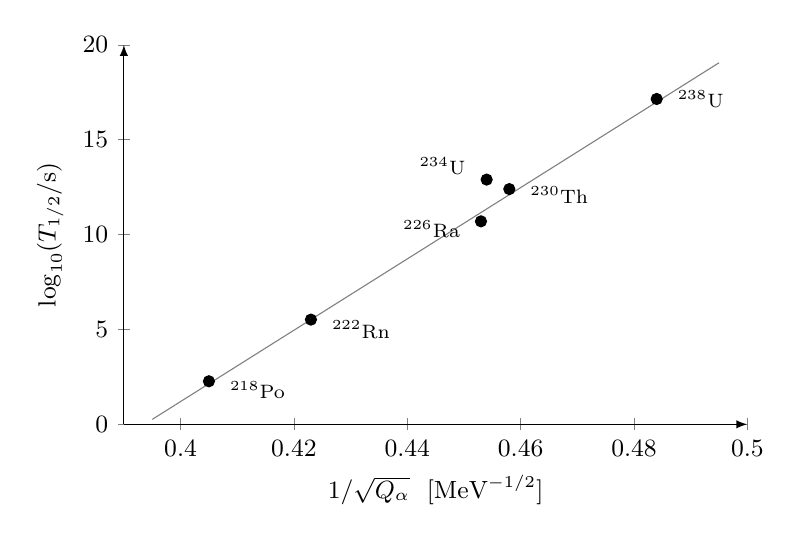
\begin{tikzpicture}
\begin{axis}[
    width=9.5cm, height=6.4cm,
    axis lines=left, axis line style={-latex},
    xlabel={$1/\sqrt{Q_\alpha}$ \ [MeV$^{-1/2}$]},
    ylabel={$\log_{10}(T_{1/2}/\mathrm{s})$},
    xlabel style={font=\small}, ylabel style={font=\small},
    tick label style={font=\small},
    xmin=0.39, xmax=0.50, ymin=0, ymax=20,
    xtick={0.40,0.42,0.44,0.46,0.48,0.50},
    ytick={0,5,10,15,20},
    clip=false,
]
\addplot[gray, thin, domain=0.395:0.495, samples=2] {188*x - 74};
\addplot[only marks, mark=*, mark size=2pt, black] coordinates {
  (0.484,17.15) (0.454,12.90) (0.458,12.40)
  (0.453,10.70) (0.423,5.52) (0.405,2.27)
};
\node[anchor=west, font=\scriptsize] at (axis cs:0.486,17.15) {$^{238}$U};
\node[anchor=east, font=\scriptsize] at (axis cs:0.452,13.6) {$^{234}$U};
\node[anchor=west, font=\scriptsize] at (axis cs:0.460,12.1) {$^{230}$Th};
\node[anchor=east, font=\scriptsize] at (axis cs:0.451,10.3) {$^{226}$Ra};
\node[anchor=west, font=\scriptsize] at (axis cs:0.425,5.0) {$^{222}$Rn};
\node[anchor=west, font=\scriptsize] at (axis cs:0.407,1.8) {$^{218}$Po};
\end{axis}
\end{tikzpicture}
\caption{Legge di Geiger-Nuttall per la serie dell'uranio.}
\label{fig:geiger_nuttall}
\end{figure}

Il punto notevole è la \emph{sensibilità}: l'energia liberata copre il modesto intervallo $4 \ \mathrm{MeV} < Q < 7 \ \mathrm{MeV}$, meno di un fattore due, mentre i tempi di dimezzamento vanno da $3 \cdot 10^{-7}$ s a $10^{10}$ anni, cioè ventiquattro ordini di grandezza. Una piccola variazione di energia ha come conseguenza una variazione enorme nella vita media, e una dipendenza così violenta suggerisce immediatamente un comportamento esponenziale.

% \section{Perché viene emessa proprio una particella \texorpdfstring{$\alpha$}{alfa}}

% Prima di fare i conti conviene capire la teoria che sta dietro, e in particolare perché fra tutti i frammenti possibili il nucleo scelga proprio l'$\alpha$.

% Consideriamo l'esempio $^{32}\mathrm{S} \to {}^{16}\mathrm{O} + {}^{16}\mathrm{O}$, sapendo che $B(^{32}\mathrm{S}) \simeq 270$ MeV. L'energia di separazione è
% %
% \begin{equation*}
%     B_{\mathrm{sep}} = 2B(^{16}\mathrm{O}) - B(^{32}\mathrm{S}) \simeq 16 \ \mathrm{MeV}
% \end{equation*}
% cioè molto più piccola dell'energia di legame totale. Questo è il punto da tenere a mente: l'energia che decide se un decadimento è permesso è una \emph{piccola differenza fra numeri grandi}, e può facilmente cambiare segno.

% Per il $^{232}\mathrm{U}$ si ottengono i valori della tabella \ref{tab:separazione}, dove un valore negativo significa che l'energia viene liberata e il decadimento è quindi energeticamente permesso.

% \begin{table}[htbp]
% \centering
% \begin{tabular}{lc|lc}
% \hline
% Frammento & $B_{\mathrm{sep}}$ [MeV] & Frammento & $B_{\mathrm{sep}}$ [MeV] \\
% \hline
% $n$ & $7,26$ & $^{4}$He & $-5,41$ \\
% $p$ & $6,12$ & $^{5}$He & $2,59$ \\
% $^{2}$H & $10,70$ & $^{6}$He & $6,19$ \\
% $^{3}$H & $10,24$ & $^{6}$Li & $3,79$ \\
% $^{3}$He & $9,92$ & $^{7}$Li & $1,94$ \\
% \hline
% \end{tabular}
% \caption{Energia necessaria per separare vari frammenti dal $^{232}\mathrm{U}$.}
% \label{tab:separazione}
% \end{table}

% L'unico valore negativo è quello dell'$^{4}\mathrm{He}$: fra tutti i frammenti leggeri, l'$\alpha$ è l'unico la cui emissione è energeticamente possibile. Il motivo è che si tratta di un nucleo eccezionalmente legato, con $B = 28,3$ MeV e $B/A = 7,07$ MeV nonostante $A = 4$, grazie al fatto di avere $Z = N = 2$ con tutti i nucleoni appaiati. È lo stesso effetto che nel capitolo precedente ha richiesto il termine di pairing nella formula semiempirica.

\subsection{La barriera coulombiana}

Il decadimento è reso possibile dalla repulsione coulombiana, che nei nuclei pesanti è talmente forte da poter espellere spontaneamente un frammento carico. Il potenziale visto dalla particella $\alpha$ è quello della figura \ref{fig:barriera}: una buca attrattiva fino al raggio di contatto $a$, e oltre quel raggio la sola repulsione coulombiana $2Ze^2/r$.

\begin{figure}[htbp]
\centering
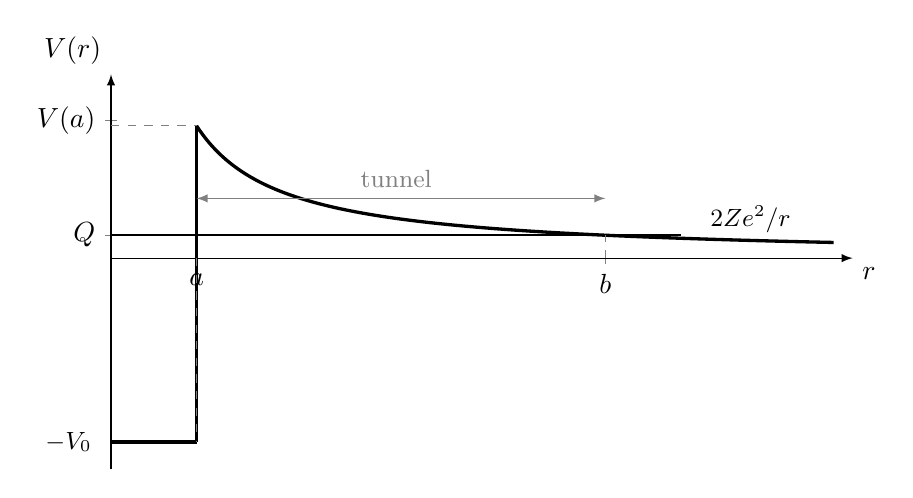
\begin{tikzpicture}
\begin{axis}[
    width=11cm, height=6.6cm,
    axis lines=middle, axis line style={-latex},
    xlabel={$r$}, ylabel={$V(r)$},
    xlabel style={at={(ticklabel* cs:1)}, anchor=north west},
    ylabel style={at={(ticklabel* cs:1)}, anchor=south east},
    xmin=0, xmax=78, ymin=-46, ymax=40,
    xtick={9,52}, xticklabels={$a$,$b$},
    ytick={5,30}, yticklabels={$Q$,$V(a)$},
    clip=false,
]
\draw[black, very thick] (axis cs:0,-40) -- (axis cs:9,-40);
\draw[black, very thick] (axis cs:9,-40) -- (axis cs:9,28.8);
\addplot[black, very thick, domain=9:76, samples=200] {259.2/x};
\draw[black, thick] (axis cs:0,5) -- (axis cs:60,5);
\draw[latex-latex, gray] (axis cs:9,13) -- (axis cs:52,13);
\node[anchor=south, font=\small, gray] at (axis cs:30,13.3) {tunnel};
\draw[dashed, gray] (axis cs:9,0) -- (axis cs:9,-40);
\draw[dashed, gray] (axis cs:52,0) -- (axis cs:52,5);
\draw[dashed, gray] (axis cs:0,28.8) -- (axis cs:9,28.8);
\node[anchor=east, font=\small] at (axis cs:-1,-40) {$-V_0$};
\node[anchor=west, font=\small] at (axis cs:62,8.5) {$2Ze^2/r$};
\end{axis}
\end{tikzpicture}
\caption{Barriera coulombiana vista dalla particella $\alpha$ nel decadimento del $^{232}\mathrm{U}$.}
\label{fig:barriera}
\end{figure}

Stimiamo i due raggi per il decadimento $^{232}_{92}\mathrm{U} \to {}^{228}_{90}\mathrm{Th} + \alpha$. Il raggio di contatto è la somma dei due raggi nucleari
%
\begin{equation*}
    a = r_0 (228)^{1/3} + R_\alpha \simeq 7,7 \ \mathrm{fm} + 1,3 \ \mathrm{fm} = 9 \ \mathrm{fm}
\end{equation*}
e l'energia coulombiana in quel punto vale, usando $e^2/\hbar c = 1/137$ e $\hbar c \simeq 200$ MeV\,fm,
%
\begin{equation*}
    V(a) = \frac{2 \cdot 90 \, e^2}{a} = 180 \cdot \frac{1}{137}\cdot\frac{200 \ \mathrm{MeV \, fm}}{9 \ \mathrm{fm}} \simeq 30 \ \mathrm{MeV}
\end{equation*}
Il raggio $b$ è invece quello a cui la barriera scende al valore dell'energia disponibile, $V(b) = Q \simeq 5$ MeV, da cui
%
\begin{equation*}
    b = \frac{2\cdot 90 \, e^2}{Q} = \frac{180}{5}\cdot\frac{200}{137} \ \mathrm{fm} \simeq 52 \ \mathrm{fm}
\end{equation*}

Il risultato è che la particella $\alpha$ esce con $5$ MeV da una barriera alta $30$ MeV. \emph{Classicamente il decadimento è impossibile}: nella regione fra $a$ e $b$ l'energia cinetica sarebbe negativa, e la particella non può trovarsi lì.

\subsection{Il modello di Gamow}

Il modello consiste nell'immaginare la particella $\alpha$ come già formata all'interno del nucleo, dove rimbalza avanti e indietro contro le pareti della buca. A ogni urto contro la barriera ha una piccola probabilità $P$ di attraversarla, per cui
%
\begin{equation}
    \lambda = \nu \cdot P
\end{equation}
dove $\nu$ è il numero di urti al secondo.

La frequenza degli urti si stima subito. Supponendo che dentro la buca la particella abbia un'energia cinetica $T \simeq 10$ MeV e usando $m_\alpha c^2 \simeq 4000$ MeV,
%
\begin{equation*}
    \frac{v}{c} = \sqrt{\frac{2T}{m_\alpha c^2}} \simeq \sqrt{\frac{20}{4000}} \simeq \frac{1}{14}
\end{equation*}
e percorrendo un tratto dell'ordine di $10$ fm fra un urto e l'altro
%
\begin{equation}
    \nu = \frac{v}{2a} \sim \frac{c}{20 \cdot 10 \ \mathrm{fm}} \simeq 1,5 \cdot 10^{21} \ \mathrm{s}^{-1}
\end{equation}

Resta da calcolare $P$, cioè la probabilità di attraversare la barriera, e qui entra in gioco tutto il capitolo. Nella regione classicamente proibita la particella si comporta come un'\emph{onda evanescente}, esattamente come il campo elettrico oltre l'interfaccia nella riflessione totale: la sua ampiezza decade esponenzialmente, e la probabilità di uscire dipende esponenzialmente dalla larghezza della barriera, cioè dalla distanza fra $a$ e $b$.

Che il meccanismo sia questo si vede già dagli ordini di grandezza. Per il $^{238}\mathrm{U}$, con $T_{1/2} = 4,47 \cdot 10^9$ anni, si ha $\lambda = \ln 2 / T_{1/2} \simeq 5 \cdot 10^{-18} \ \mathrm{s}^{-1}$, da cui
%
\begin{equation*}
    P = \frac{\lambda}{\nu} \sim 10^{-39}
\end{equation*}
La particella $\alpha$ urta la barriera $10^{21}$ volte al secondo per miliardi di anni, e a ogni tentativo ha una probabilità su $10^{39}$ di passare. Soltanto una dipendenza esponenziale può produrre numeri del genere, ed è proprio questa dipendenza a spiegare la legge di Geiger-Nuttall \eqref{eq:geiger_nuttall}: una piccola variazione di $Q$ sposta $b$, cambia la larghezza della barriera e modifica di molti ordini di grandezza la vita media

Non ci resta che trovare una forma esplicita per $P$.

\subsection*{Effetto tunnel per potenziale rettangolare}

Prima di passare al caso di nostro interesse, consideriamo quello in cui il potenziale considerato ha una forma rettangolare e si ha $E < V_0$.

\begin{figure}[h]
    \centering
    \begin{tikzpicture}[>=Stealth, scale=1.1]

    % zona 2 ombreggiata
    \fill[black!8] (0,0) rectangle (3.5,3);

    % separatori verticali
    \draw[dotted, black!55] (0,0) -- (0,4.4);
    \draw[dotted, black!55] (3.5,0) -- (3.5,4.4);

    % assi
    \draw[->] (-3.6,0) -- (7.9,0) node[below] {$x$};
    \draw[->] (-3.6,0) -- (-3.6,4.55) node[left] {$V(x)$};

    % potenziale
    \draw[very thick] (-3.6,0) -- (0,0) -- (0,3) -- (3.5,3) -- (3.5,0) -- (7.7,0);

    % tacche sull'asse verticale
    \draw (-3.72,3) -- (-3.6,3);
    \node[anchor=east, font=\small] at (-3.74,3) {$V_0$};
    \draw (-3.72,1.35) -- (-3.6,1.35);
    \node[anchor=east, font=\small] at (-3.74,1.35) {$E$};

    % livello energetico
    \draw[dashed] (-3.6,1.35) -- (7.7,1.35);

    % larghezza della barriera
    \draw[<->] (0,-0.8) -- (3.5,-0.8);
    \node[anchor=north, font=\small] at (1.75,-0.84) {$L = x_1 - x_0$};

    % etichette delle zone
    \node[font=\small] at (-1.8,4.25) {zona 1};
    \node[font=\small] at (1.75,4.25) {zona 2};
    \node[font=\small] at (5.6,4.25) {zona 3};

    % numeri d'onda
    \node[font=\small] at (-1.8,3.55) {$k = \dfrac{\sqrt{2mE}}{\hbar}$};
    \node[font=\small] at (1.75,3.55) {$k_0 = \dfrac{\sqrt{2m(V_0-E)}}{\hbar}$};
    \node[font=\small] at (5.6,3.55) {$k = \dfrac{\sqrt{2mE}}{\hbar}$};

    % comportamento della soluzione
    \node[font=\small] at (-1.8,0.7) {$\psi \sim e^{\pm ikx}$};
    \node[font=\small] at (1.75,0.7) {$\psi \sim e^{\pm k_0 x}$};
    \node[font=\small] at (5.6,0.7) {$\psi \sim e^{ikx}$};

    % punti sull'asse
    \node[anchor=north, font=\small] at (0,-0.08) {$x_0$};
    \node[anchor=north, font=\small] at (3.5,-0.08) {$x_1$};

    \end{tikzpicture}
    \caption{Barriera di potenziale rettangolare di altezza $V_0$ ed estensione $L$, con una particella di energia $E < V_0$.}
    \label{fig:barriera_potenziale}
\end{figure}

Cosniderando gli autostati dell'hamiltoniano, l'equazione di Schrödinger in coordinate è 
%
\begin{equation}
    \left( -\frac{\hbar^2}{2 m} \frac{d^2}{dx^2} + V'\right) \psi_E(x) = E \psi_E(x)
\end{equation}
Dove si ha che $V' = 0$ nelle zone $1$ e $3$, mentre $V' = V_0$ nella zona $2$. \\
Risolvendo l'equazione si ottengono le soluzioni nella forma 
%
\begin{align}
    \psi_E(x) &= Ae^{ikx} + Be^{-ikx} \quad x < x_0\\
    \psi_E(x) &= Ce^{k_0 x} + D e^{- k_0 x} \quad x_0 < x < x_1\\
    \psi_E(x) &= Fe^{i k x} \quad \qquad \qquad x > x_1 
\end{align}
Dove abbiamo posto 
%
\begin{equation}
    k_0 = \sqrt{\frac{2m}{\hbar^2} (V_0 - E)} \quad, \quad k = \sqrt{\frac{2m}{\hbar^2}E}
\end{equation}
In particolare si può notare dal verso di propogazione che, se ci immaginiamo un fascio di particelle sparate da sinistra verso il potenziale, $|A|^2$ rappresenta il numero di particelle incidenti, $|B|^2$ il numero di particelle riflesse e $|F|^2$ il numero di particelle trasmesse. Deve quindi valere la relazione 
%
\begin{equation*}
    |F|^2 + |B|^2= |A|^2
\end{equation*}
Da qui è facile intuire che la probabilità che la particella attraversi il potenziale sia proprio 
%
\begin{equation}
    P = \frac{|F|^2}{|A|^2}
\end{equation}

\'E possibile trovare una relazione tra $A, B, C, D, F$ imponendo la continuità della funzione d'onda e della sua derivata nei punti $x_0$ e $x_1$, quindi, imponendo $4$ condizioni, è possibile rappresentrare tutti i parametri in funzione di $A$, in particolare si ottiene 
%
\begin{equation*}
    |F|^2 = \frac{|A|^2}{1+\frac{V_0^2}{4 E\left(V_0-E\right)} \sinh ^2 k_0 L}
\end{equation*}
Cosa che implica che 
\begin{equation*}
    P = \frac{1}{1+\frac{V_0^2}{4 E\left(V_0-E\right)} \sinh ^2 k_0 L}
\end{equation*}
Sviluppando $\sinh^2 k_0 L = 1/4 (e^{2 k_0 L} - 2 + e^{-2k_0 L}) \approx 1/4 \ e^{2 k_0 L}$ si ottiene
\begin{equation}
    P \propto \text{exp}\left( -2 L \sqrt{\frac{2m}{\hbar^2} (V_0 - E)} \right)
\end{equation}

\subsection*{Effetto tunnel per un potenziale qualunque}

Passiamo adesso al nostro caso. \\
Un potenziale generico $V(r)$ può essere visto come una sequenza di una serie di barriere infinitesime, ciascuna con probabilità di essere attraversata
\begin{equation}
    P_{\text{inf}} \propto \text{exp}\left( -2 \sqrt{\frac{2m}{\hbar^2} (V(r) - Q) } \ dr  \right)
\end{equation}
La probabilità di attraversare la barriera completa è data dal prodotto delle probabilità di attraversare le barriere infinitesimali
\begin{tcolorbox}[colback=black!5!white, colframe=black!45!white, boxrule=0.8pt]
\begin{equation}
    P \propto \text{exp}\left( -2 \int_{a}^{b}\sqrt{\frac{2m}{\hbar^2} (V(r) - Q) } \ dr  \right)
\end{equation}
\end{tcolorbox}

Ovvero vale $P \propto e^{-2G}$ dove $G$ prende il nome di fattore di Gamow\mkeyword{fattore di Gamow} e quindi 
\begin{tcolorbox}[colback=black!5!white, colframe=black!45!white, boxrule=0.8pt]
\begin{equation}
    G = \int_{a}^{b} \sqrt{\frac{2m}{\hbar^2} (V(r) - Q)} \ dr
\end{equation}
\end{tcolorbox}

Gli estremi di integrazione delimitano la regione classicamente proibita: $a$ è il raggio nucleare, dove la barriera comincia, e $b$ è il punto di inversione esterno, definito da $V(b) = Q$.

\subsection*{Il fattore di Gamow per la barriera coulombiana}

Applichiamo il risultato generale al nostro potenziale, $V(r) = \dfrac{zZe^2}{r}$, dove $z = 2$ è la carica della particella $\alpha$ e $Z$ quella del nucleo \emph{figlio}. Conviene anzitutto eliminare la costante $zZe^2$ in favore del punto di inversione esterno: dalla sua definizione $V(b) = Q$ segue $zZe^2 = Q\,b$, e quindi
%
\begin{equation*}
    V(r) - Q = \frac{zZe^2}{r} - Q = Q\left(\frac{b}{r} - 1\right)
\end{equation*}
Sostituendo nel fattore di Gamow si ottiene
%
\begin{equation}
    G = \frac{\sqrt{2mQ}}{\hbar}\int_a^b \sqrt{\frac{b}{r} - 1} \; dr
    \label{eq:G_coulomb}
\end{equation}
dove tutta la dipendenza dai parametri del nucleo è ormai confinata nel prefattore e negli estremi. Poniamo adesso $\xi = r/b$, da cui $dr = b \, d\xi$ e gli estremi diventano $a/b$ e $1$,
%
\begin{equation}
    G = \frac{\sqrt{2mQ}}{\hbar}\,b \int_{a/b}^{1} \sqrt{\frac{1}{\xi} - 1} \; d\xi = \frac{zZe^2\sqrt{2m}}{\hbar \sqrt{Q}} \int_{a/b}^{1} \sqrt{\frac{1}{\xi} - 1} \; d\xi
    \label{eq:G_adimensionale}
\end{equation}
avendo riusato $b = zZe^2/Q$ nell'ultimo passaggio. L'integrale è adesso un numero puro che dipende dal solo rapporto $a/b$.\\

Per calcolarlo si pone $\xi = \sin^2\theta$, cosicché $d\xi = 2\sin\theta\cos\theta \, d\theta$ e l'integrando diventa
%
\begin{equation*}
    \sqrt{\frac{1-\sin^2\theta}{\sin^2\theta}} \cdot 2\sin\theta\cos\theta \, d\theta = 2\cos^2\theta \, d\theta = \left(1 + \cos 2\theta\right) d\theta
\end{equation*}
che si integra immediatamente in $\theta + \sin\theta\cos\theta$. Tornando alla variabile originaria si ottiene
%
\begin{equation}
    \int_{c}^{1} \sqrt{\frac{1}{\xi} - 1} \; d\xi = \arccos\sqrt{c} - \sqrt{c\left(1-c\right)}
    \label{eq:integrale_notevole}
\end{equation}

Nel nostro caso $c = a/b$ è piccolo: per il $^{238}\mathrm{U}$, con $Q = 4{,}27$ MeV, si ha $b = zZe^2/Q \simeq 61$ fm contro $a \simeq 9$ fm, cioè $a/b \simeq 0{,}15$. Possiamo allora sviluppare, usando $\arccos x \simeq \pi/2 - x$ e $\sqrt{c(1-c)} \simeq \sqrt{c}$,
%
\begin{equation}
    \arccos\sqrt{\frac{a}{b}} - \sqrt{\frac{a}{b}\left(1 - \frac{a}{b}\right)} \ \simeq \ \frac{\pi}{2} - 2\sqrt{\frac{a}{b}} = \frac{\pi}{2} - 2\sqrt{\frac{aQ}{zZe^2}}
    \label{eq:sviluppo}
\end{equation}
Sostituendo nella \eqref{eq:G_adimensionale}, il secondo termine cancella la dipendenza da $Q$ e si arriva al risultato centrale del capitolo

\begin{tcolorbox}[colback=black!5!white, colframe=black!45!white, boxrule=0.8pt]
\begin{equation}
    G = \frac{c_1}{\sqrt{Q}} - c_2 \qquad , \qquad c_1 = \frac{\pi}{2}\, zZ\alpha \sqrt{2mc^2} \qquad , \qquad c_2 = 2\sqrt{\frac{2mc^2 \, zZ\alpha \, a}{\hbar c}}
    \label{eq:G_finale}
\end{equation}
\end{tcolorbox}
Le due costanti dipendono dal nuclide ma \emph{non} dall'energia: tutta la dipendenza da $Q$ è nel primo termine, ed è del tipo $Q^{-1/2}$. Si noti anche che $c_2$ contiene il raggio di contatto $a$, mentre $c_1$ no: è il termine che corregge il fatto che la barriera non viene attraversata da zero ma a partire dalla superficie nucleare.\\

\subsection*{La legge di Geiger-Nuttall}

A questo punto la costante di decadimento è completamente determinata. Inserendo la \eqref{eq:G_finale} in $\lambda = \nu P$ e passando alla vita media si ottiene
%
\begin{equation}
    \tau = \frac{1}{\lambda} = \frac{1}{\nu}\, e^{2G} = \frac{1}{\nu}\exp\left(\frac{2c_1}{\sqrt{Q}} - 2c_2\right)
    \label{eq:tau_gamow}
\end{equation}
e prendendo il logaritmo

\begin{tcolorbox}[colback=black!5!white, colframe=black!45!white, boxrule=0.8pt]
\begin{equation}
    \ln \tau = \frac{2c_1}{\sqrt{Q}} - \left(2c_2 + \ln \nu\right)
    \label{eq:GN_derivata}
\end{equation}
\end{tcolorbox}
che è esattamente la forma della legge di Geiger-Nuttall \eqref{eq:geiger_nuttall} osservata sperimentalmente. Il dato empirico da cui eravamo partiti è così spiegato: la retta nel piano $(1/\sqrt{Q}, \log T_{1/2})$ non è una coincidenza, ma il logaritmo di una probabilità di tunneling.\\